\subsection{Aplikacja Poszkodowanego - Symulacja Funkcji Życiowych Pacjenta }
\subsubsection{Data}
25.03
\subsubsection{Osoby odpowiedzialne}
Adrian Winiarski, Szymon Klimczuk

\subsubsection{Specyfikacja}
\begin{itemize}
    \item{Symulowane są 2 funkcje życiowe - puls oraz oddech}
    \item{Sygnały generowane muszą być niezależne od reszty aplikacji}
    \item Generowany sygnał odpowiada stopniowi obrażeń poszkodowanego
\newline
\newline
 Na zdjęciach poniżej są pokazane 3 interfejsy. Na pierwszym mamy interfejs główny. Drugi interfejs z rozwinięta listą w której można skategoryzować pacjenta wybierając odpowiedni kolor do wyboru mamy 4 podstawowe czyli: czarny, czerwony, zielony, żółty.
\begin{figure}[h!]
  \centering
    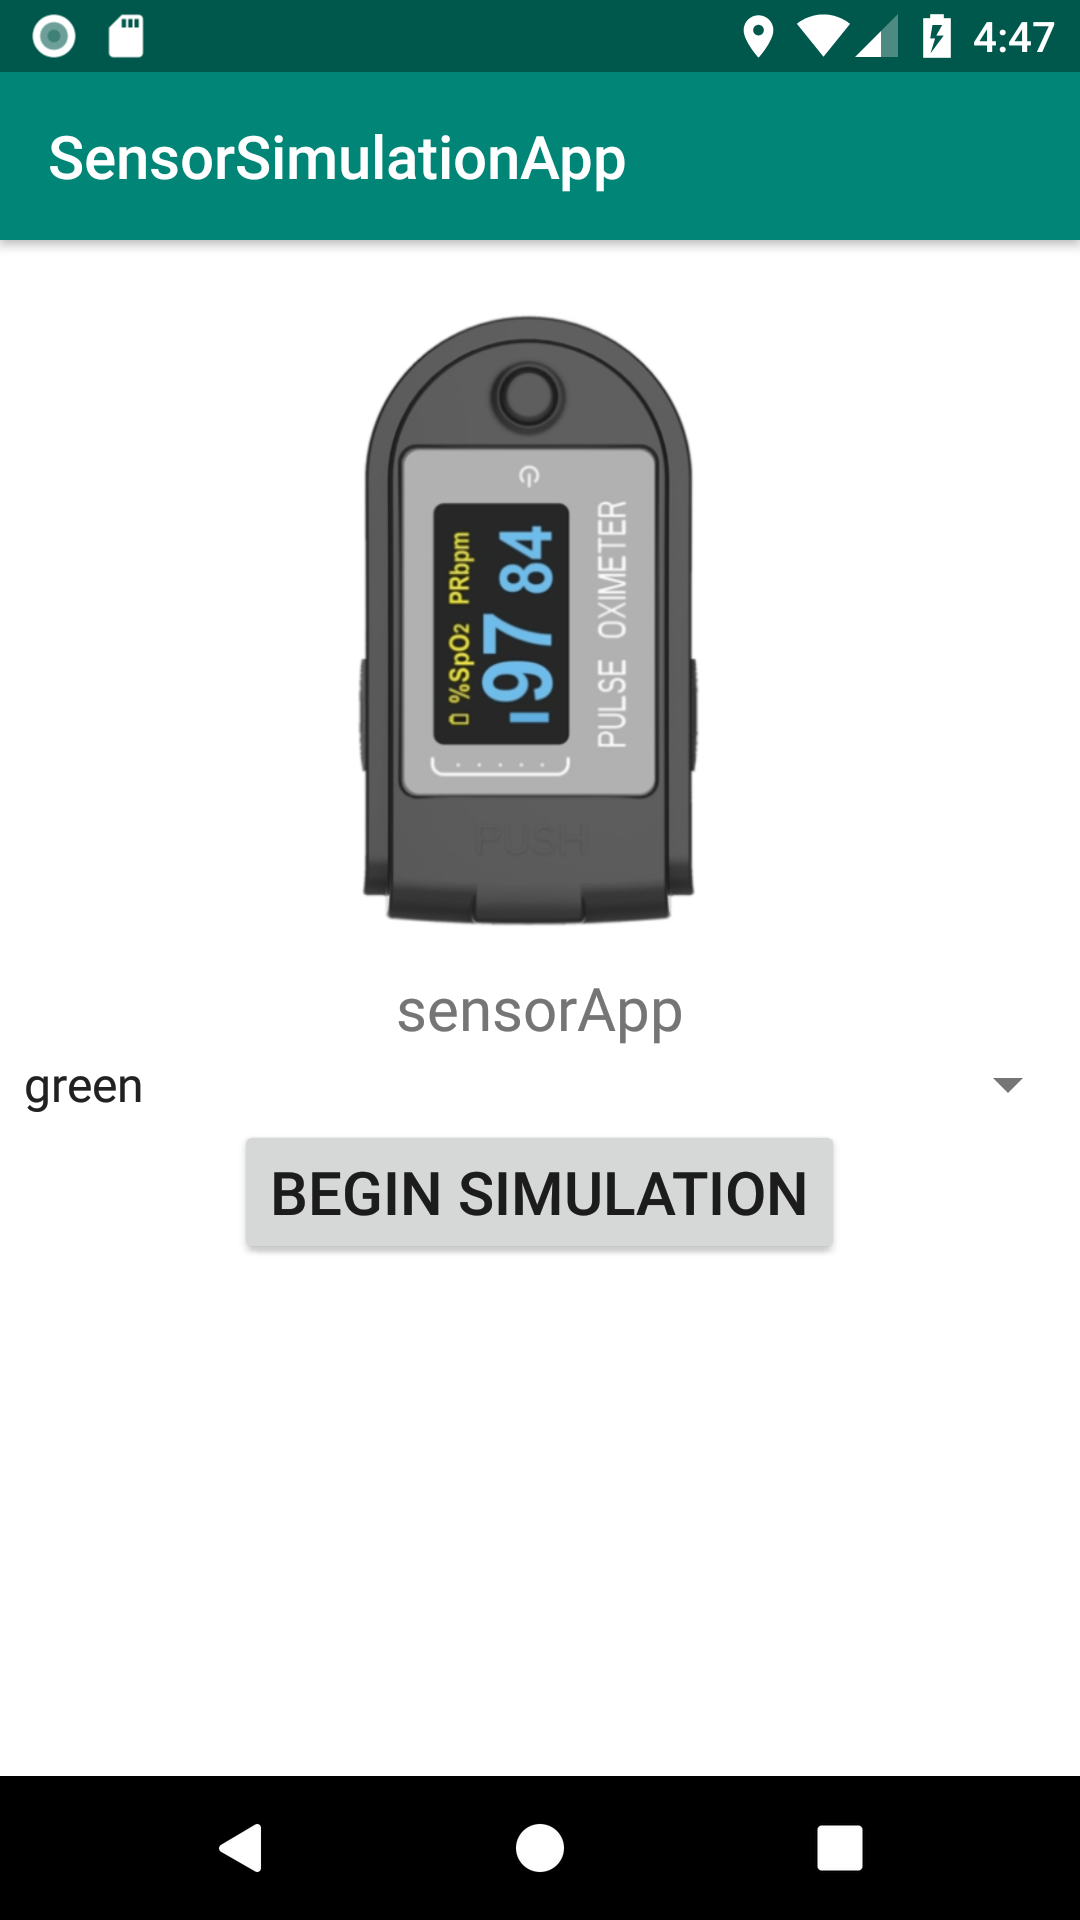
\includegraphics[width=0.30\textwidth]{img/start.png}
  \caption{Główny ekran} 
  \label{fig:org}                                       
\end{figure}
\end{itemize}
\newpage
\begin{figure}[h!]
  \centering
    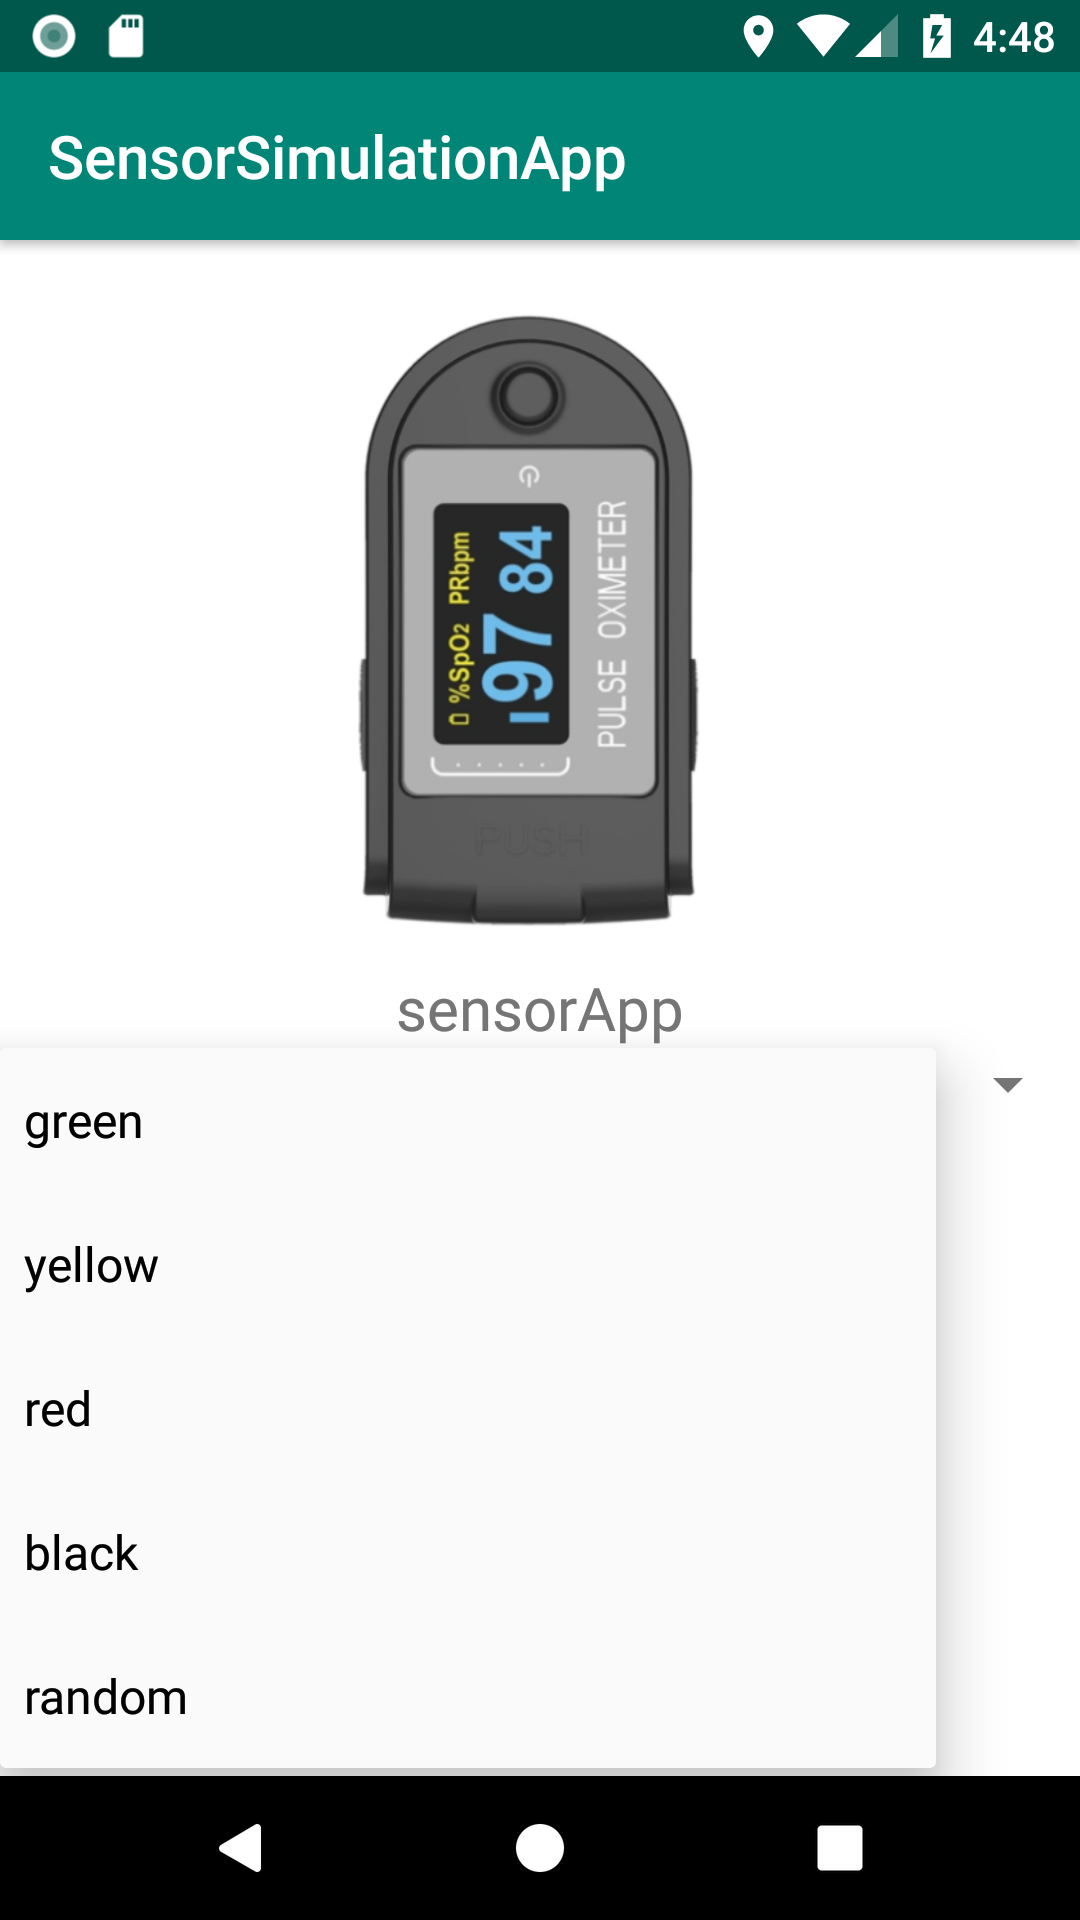
\includegraphics[width=0.30\textwidth]{img/scroll.png}
  \caption{Ekran z rozwiniętą listą} 
  \label{fig:org}                                       
\end{figure}
\begin{figure}[h!]
  \centering
    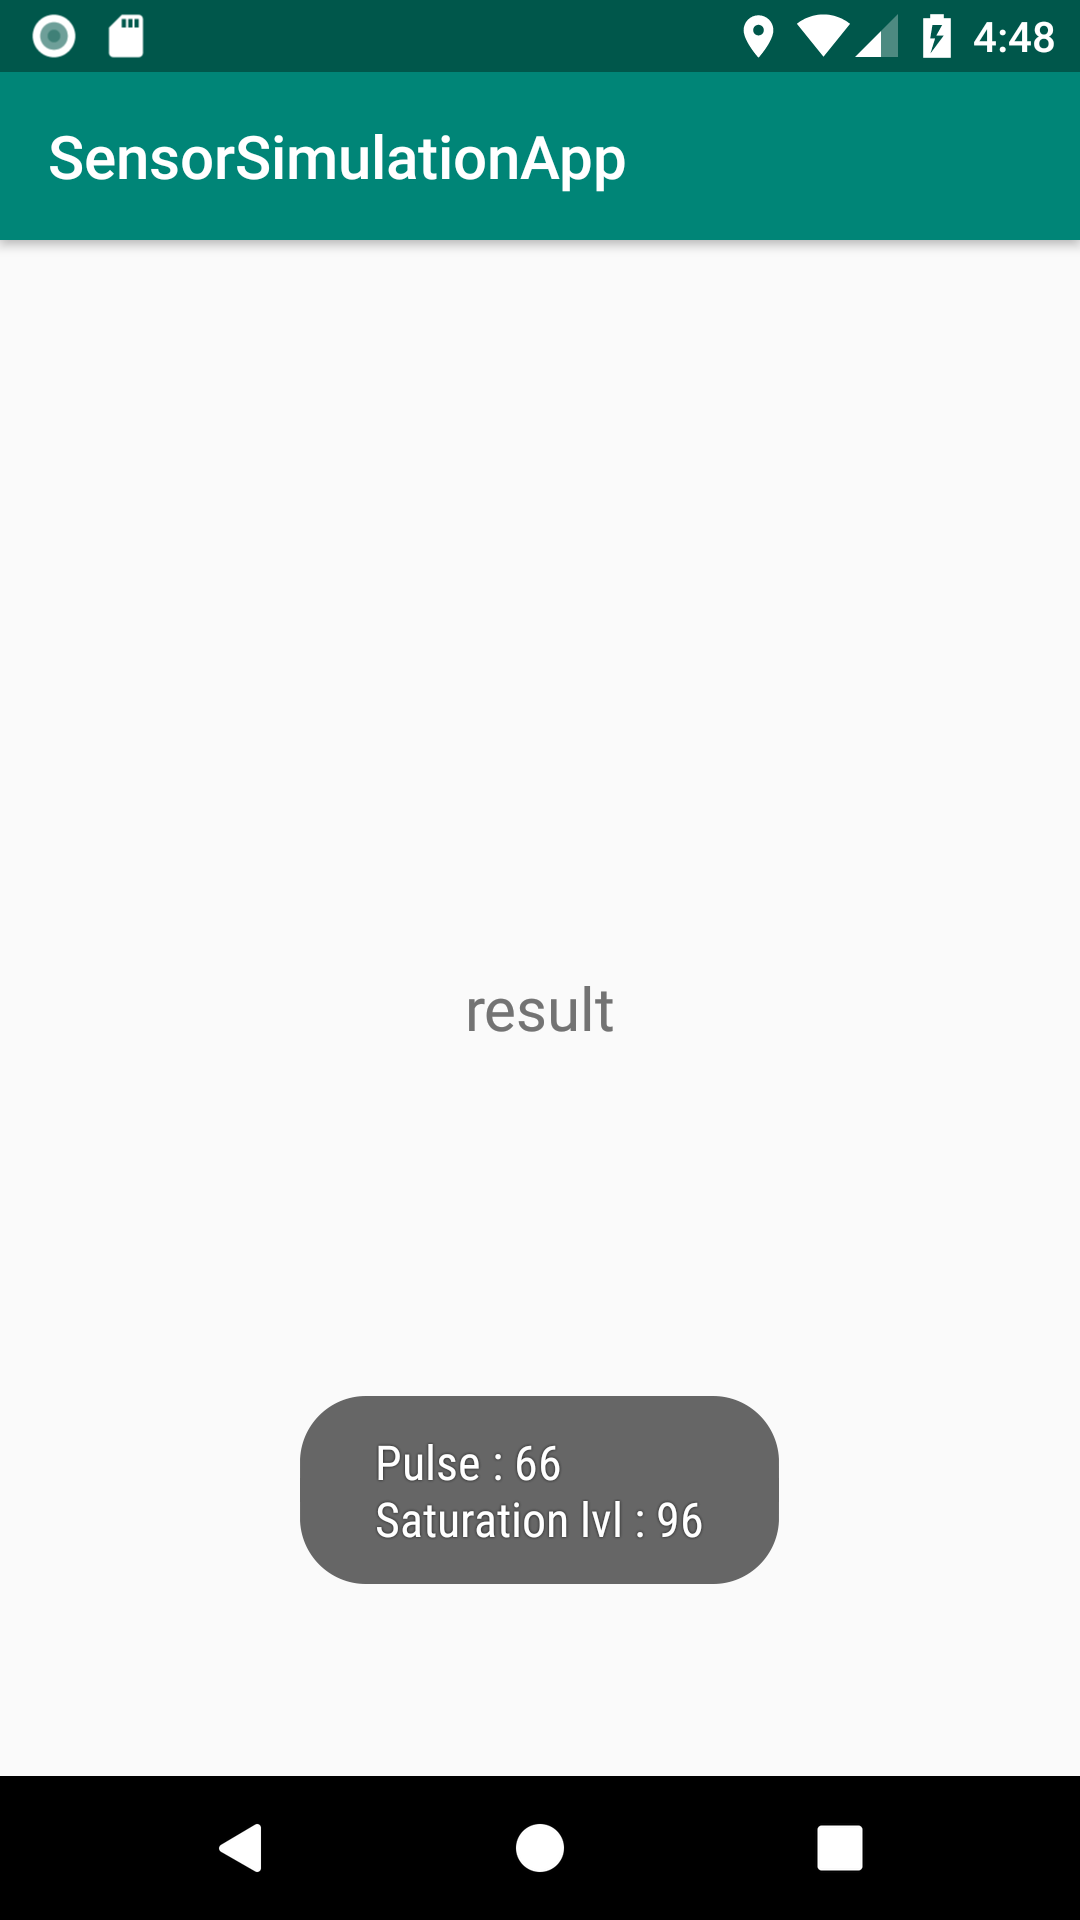
\includegraphics[width=0.30\textwidth]{img/result.png}
  \caption{Ekran z symulowaną saturacją i pulsem} 
  \label{fig:org}                                       
\end{figure}

\subsubsection{Wymagania zewnętrzne}

